\section{Introduction to Linear Quadratic Regulator (LQR)}
\subsection{LQR Problem}
\begin{equation}
    \begin{aligned}
        \min_{\substack{x_{1:N}\\u_{1:N-1}}}J=\sum_{k=1}^{N-1}{\frac{1}{2}x_{k}^{T}Q_kx_k+\frac{1}{2}u_{k}^{T}R_ku_k}+\frac{1}{2}x_{N}^{T}Q_Nx_N \\
        \text{s.t.} \qquad x_{k+1} = A_k x_k + B_k u_k \\
        Q \succeq 0, R \succ 0 
    \end{aligned}
\end{equation}
\begin{itemize}
    \item Can (locally) approximate many nonlinear problems.
    \item Computationally tractable.
    \item Many extensions, e.g. infinite horizon, stochastic and etc.
    \item ``Time invariant'' if $A_k =A, B_k =B, Q_k=Q, R_k=R, \forall t$, ``time varying'' otherwise.
\end{itemize}

\subsection{LQR with Indirect Shooting}

From Pontryagin's maximum (minimum) principle, we can derive the KKT conditions for LQR problem:
\begin{equation}
    \begin{aligned}
        x_{k+1}=\nabla _{\lambda}H\left( x_k,u_k,\lambda _{k+1} \right) =Ax_k+Bu_k\\
        \lambda _k=\nabla _xH\left( x_k,u_k,\lambda _{k+1} \right) =Qx_k+A^T\lambda _{k+1}\\
        \lambda _N=Q_Nx_N\\
        u_k=\text{arg}\min _{\tilde{u}}H\left( x_k,\tilde{u},\lambda _{k+1} \right) = -R^{-1}B^T\lambda_{k+1}\\
    \end{aligned}
\end{equation}

\begin{itemize}
    \item Procedure:
    \begin{algorithmic}[1]
        \STATE Start with an initial guess $u_{1:N-1}$ trajectory.
        \STATE Simulate / ``rollout'' to get $x_{1:N}$.
        \STATE Backward pass to get $\lambda$ and $\Delta u$.
        \STATE Rollout with line search on $\Delta u$.
        \STATE Goto 3 until convergence. 
    \end{algorithmic}
    \item This is doing gradient descent on the $u$ and this is just a recipe for computing the gradients efficiently by back propagation through the Dynamics so it's like back propagation in a neural network, but it's through time, through the Dynamics instead of the NN layers.
    \item Just for clarification: the primal variable is $u$, so do the same trick as before (Newton's method, line search, etc.).
    \item Convergence condition should be considered. I choose $\Delta J$ in the programme.
    \item Example -- Double Integrator (Think of this as a brick sliding on ice without friction):
    \begin{equation}
        \dot{x}=\left[ \begin{array}{c}
            \dot{q}\\
            \ddot{q}\\
        \end{array} \right] =\left[ \begin{matrix}
            0&		1\\
            0&		0\\
        \end{matrix} \right] \left[ \begin{array}{c}
            q\\
            \dot{q}\\
        \end{array} \right] +\left[ \begin{array}{c}
            0\\
            1\\
        \end{array} \right] u
    \end{equation}
    in which $q, \dot q, \ddot q$ stands for position, velocity and acceleration respectively. The system can be discretized using matrix exponential:
    \begin{equation}
        x_{k+1}=\left[ \begin{matrix}
            1&		h\\
            0&		1\\
        \end{matrix} \right] \left[ \begin{array}{c}
            q_k\\
            \dot{q}_k\\
        \end{array} \right] +\left[ \begin{array}{c}
            \frac{1}{2}h^2\\
            h\\
        \end{array} \right] u_k
    \end{equation}
    \item Result: When the horizon goes longer, the computational cost grows superlinearly. For example, change horizon from 5s to 20s, the number of iterations has increased by far more than four times.
    \item Analysis: This is like the control version of the gradient vanishing and exploding phenomena in deep learning. The control lingo term for this is the ``tail wagging the dog problem''. Basically if you have really long horizon and you're doing this backward recursion, you'll error compounding and gradients get nasty.
    \item This is a linear problem, which should be easy to guess, but it still kind of sucks here so if you try this on a non-linear problem, these methods get really nasty and don't work well.
\end{itemize}

\subsection{LQR as QP}

This is more effective than direct shooting method. Assuming $x_1$ (initial state) is given (not a decision variable). We do some definitions first:

Control-State sequence (similar to action-state sequence in reinforcement learning):
\begin{equation}
    z=\left[ \begin{array}{c}
        u_1\\
        x_2\\
        u_2\\
        x_3\\
        \vdots\\
        x_N\\
    \end{array} \right] 
\end{equation}

Quadratic matrix:
\begin{equation}
    H=\left[ \begin{matrix}
        R_1&		&		&		&		&		\\
        &		Q_2&		&		&		&		\\
        &		&		R_2&		&		&		\\
        &		&		&		Q_3&		&		\\
        &		&		&		&		\ddots&		\\
        &		&		&		&		&		Q_N\\
    \end{matrix} \right] 
\end{equation}

Therefore, the cost function can be written as:
\begin{equation}
    J=\frac{1}{2}z^THz
\end{equation}

Define $C$ and $d$:
\begin{equation}
    \underset{C}{\underbrace{\left[ \begin{matrix}
        B&		-I&		0&		&		&		&		&		\\
        &		A&		B&		-I&		0&		&		&		\\
        &		&		&		\ddots&		&		&		&		\\
        &		&		&		&		&		A_{N-1}&		B_{N-1}&		-I\\
    \end{matrix} \right] }}\underset{z}{\underbrace{\left[ \begin{array}{c}
        u_1\\
        x_2\\
        u_2\\
        x_3\\
        \vdots\\
        x_N\\
    \end{array} \right] }}=\underset{d}{\underbrace{\left[ \begin{array}{c}
        -Ax_1\\
        0\\
        0\\
        \vdots\\
        0\\
    \end{array} \right] }}
\end{equation}

Now the LQR problem is formulated as a standard QP problem. The Lagrangian of this QP is:
\begin{equation}
    L(z,\lambda) = \frac{1}{2}z^THz+\lambda^T(Cz-d)
\end{equation}

KKT conditions:
\begin{equation}
    \begin{array}{c}
        \nabla _zL=Hz+C^T\lambda =0\\
        \nabla _{\lambda}L=Cz-d=0\\
    \end{array}\Rightarrow \left[ \begin{matrix}
        H&		C^T\\
        C&		0\\
    \end{matrix} \right] \left[ \begin{array}{c}
        z\\
        \lambda\\
    \end{array} \right] =\left[ \begin{array}{c}
        0\\
        d\\
    \end{array} \right] 
\end{equation}

How many iterations of Newton's method do I need to solve this problem? One. It's a linear problem, so we can get the exact (close-form, analytic) solution by solving a linear system. Just go and play with coding, try different parameters. You will find QP is much better than shooting. (10 times bigger matrix, but no more complex computation. Why? We'll take a closer look at LQR-QP later)

\subsection{Riccati Equation}
\begin{equation}
    \left[ \begin{array}{cccccc:ccc}
        R&		&		&		&		&		&		B^T&		&		\\
        &		Q&		&		&		&		&		-I&		A^{-1}&		\\
        &		&		R&		&		&		&		&		B^{-1}&		\\
        \arrayrulecolor{green}\hdashline
        &		&		&		\textcolor{green}{Q}&		&		&		&		\textcolor{green}{-I}&		\textcolor{green}{A}\\
        \arrayrulecolor{red}\hdashline
        &		&		&		&		\textcolor{red}{R}&		&		&		&		\textcolor{red}{B^T}\\
        \arrayrulecolor{blue}\hdashline
        &		&		&		&		&		\textcolor{blue}{Q_N}&		&		&		\textcolor{blue}{-I}\\
        \arrayrulecolor{black}\hdashline
        B&		-I&		&		&		&		&		&		&		\\
        &		A&		B&		-I&		&		&		&		0&		\\
        &		&		&		A&		B&		-I&		&		&		\\
    \end{array} \right] \left[ \begin{array}{c}
        u_1\\
        x_2\\
        u_2\\
        \arrayrulecolor{green}\hdashline
        \textcolor{green}{x_3}\\
        \arrayrulecolor{red}\hdashline
        \textcolor{red}{u_3}\\
        \arrayrulecolor{blue}\hdashline
        \textcolor{blue}{x_4}\\
        \arrayrulecolor{black}\hdashline
        \lambda _2\\
        \lambda _3\\
        \lambda _4\\
    \end{array} \right] =\left[ \begin{array}{c}
        0\\
        0\\
        0\\
        \arrayrulecolor{green}\hdashline
        \textcolor{green}{0}\\
        \arrayrulecolor{red}\hdashline
        \textcolor{red}{0}\\
        \arrayrulecolor{blue}\hdashline
        \textcolor{blue}{0}\\
        \arrayrulecolor{black}\hdashline
        -Ax_1\\
        0\\
        0\\
    \end{array} \right] 
\end{equation}

The KKT system for LQR is very sparse (lots of zeros) and has a lot of structure, so we have some tricks to solve it efficiently. The trick we use is the ``back substitution'' in linear algebra (like solving triangular matrices). We can make the following deductions in sequence:
\begin{equation}
    \centering
    \begin{array}{l}
        \textcolor{blue}{Q_Nx_4-\lambda _4=0\Rightarrow \lambda _4=Q_Nx_4}\\
        \textcolor{red}{Ru_3+B^T\lambda _4=Ru_3+B^TQ_Nx_4=Ru_3+B^TQ_N\left( Ax_3+Bu_3 \right) =0}\\
        \textcolor{red}{\Rightarrow u_3=-\underset{K_3}{\underbrace{\left( R+B^TQ_NB \right) ^{-1}B^TQ_NA}}x_3}\\
        \textcolor{green}{Qx_3-\lambda _3+A^T\lambda _4=Qx_3-\lambda _3+A^TQ_Nx_4=Qx_3-\lambda _3+A^TQ_N\left( Ax_3+Bu_3 \right) =0}\\
        \textcolor{green}{\Rightarrow \lambda _3=\underset{P_3}{\underbrace{\left( Q+A^TQ_N\left( A-BK \right) \right) }}x_3}\\
    \end{array}
\end{equation}
Now we have a recursion for $K$ and $P$:
\begin{equation}
    \begin{aligned}
        P_N=Q_N\\
        K_k=\left( R+B^TP_{k+1}B \right) ^{-1}B^TP_{k+1}A\\
        P_k=Q+A^TP_{k+1}\left( A-BK_k \right)\\
    \end{aligned}
    \label{equ:riccati-recursion}
\end{equation}

This is called the Riccati equation/recursion. We can solve the QP by doing a backward Riccati recursion followed by a forward rollout to compute $x_{1:N}$ and $u_{1:N-1}$ from initial conditions. A general (dense) QP has complexity $O(N^3(n+m)^3)$, $N$ is time horizon, $n$ is state dim, $m$ is control dim, while Riccati solution is $O(N(n+m)^3)$.

Even more important: we now have a feedback policy $u=-Kx$ instead of an open-loop trajectory. 

Example shows that (Just go and play with coding, try different parameters):
\begin{itemize}
    \item Riccati solution exactly matches QP solution.
    \item Feedback policy lets us change $x_0$ and reject noise / disturbances.
    \item Independent of $x,u$. It offers a global feedback policy that works anywhere from any initial condition.
    \item continuous-time version is very hard to handle.
    \item Comparing to shooting method, LQR-QP and Riccati Recursion do not require a initial guess for $u$, which is awesome.
\end{itemize}

\subsection{Infinite Horizon LQR}
From the example, we find out that matrix $K$ converges to a constant matrix as $k$ increases. Therefore, for an infinite time domain LQR system, the resulting $K$ will be a constant matrix. For a stabilization problem, we usually use this constant matrix $K$ directly. If we call the LQR function in MATLAB or Julia, we will return an optimal feedback control $K$ (in this section, it is actually an optimal PD controller). The close-loop system turn out to be stable.

From Riccati recursion in Equ. \eqref{equ:riccati-recursion}, the infinite-horizon limit $P_{k} = P_{k+1} = P_{\infty}$, which can be solved as a root-finding/fixed-point problem. Julia/Matlab/Python has ``dare'' function do this for you.

\section{Supplement 4}
\subsection{Review on LQR}
Our discrete time dynamics is a Markov Decision Process (MDP). Basically we have states and actions, and we need a state and action to get to the next state. Because of this, our finite control problems deal with N $x$, and (N-1) $u$.

\begin{center}
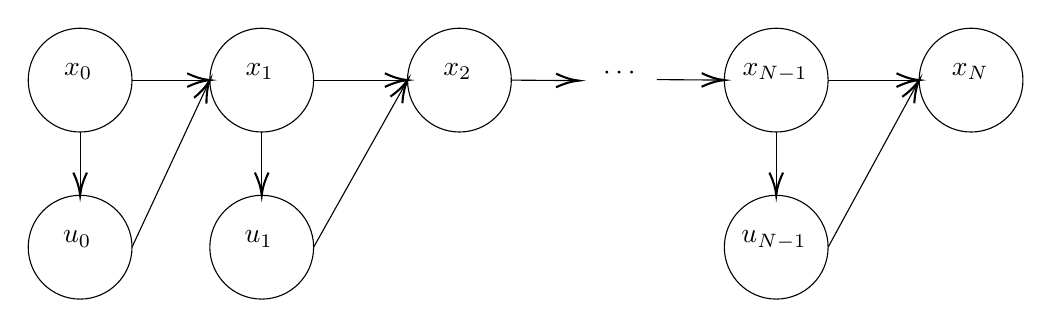
\begin{tikzpicture}[x=0.75pt,y=0.75pt,yscale=-1,xscale=1]
\draw   (50.25,103.25) .. controls (50.25,89.44) and (61.44,78.25) .. (75.25,78.25) .. controls (89.06,78.25) and (100.25,89.44) .. (100.25,103.25) .. controls (100.25,117.06) and (89.06,128.25) .. (75.25,128.25) .. controls (61.44,128.25) and (50.25,117.06) .. (50.25,103.25) -- cycle ;
\draw   (50.25,183.75) .. controls (50.25,169.94) and (61.44,158.75) .. (75.25,158.75) .. controls (89.06,158.75) and (100.25,169.94) .. (100.25,183.75) .. controls (100.25,197.56) and (89.06,208.75) .. (75.25,208.75) .. controls (61.44,208.75) and (50.25,197.56) .. (50.25,183.75) -- cycle ;
\draw   (137.75,183.75) .. controls (137.75,169.94) and (148.94,158.75) .. (162.75,158.75) .. controls (176.56,158.75) and (187.75,169.94) .. (187.75,183.75) .. controls (187.75,197.56) and (176.56,208.75) .. (162.75,208.75) .. controls (148.94,208.75) and (137.75,197.56) .. (137.75,183.75) -- cycle ;
\draw   (233,103.25) .. controls (233,89.44) and (244.19,78.25) .. (258,78.25) .. controls (271.81,78.25) and (283,89.44) .. (283,103.25) .. controls (283,117.06) and (271.81,128.25) .. (258,128.25) .. controls (244.19,128.25) and (233,117.06) .. (233,103.25) -- cycle ;
\draw   (137.75,103.25) .. controls (137.75,89.44) and (148.94,78.25) .. (162.75,78.25) .. controls (176.56,78.25) and (187.75,89.44) .. (187.75,103.25) .. controls (187.75,117.06) and (176.56,128.25) .. (162.75,128.25) .. controls (148.94,128.25) and (137.75,117.06) .. (137.75,103.25) -- cycle ;
\draw   (385.63,183.75) .. controls (385.63,169.94) and (396.82,158.75) .. (410.63,158.75) .. controls (424.43,158.75) and (435.63,169.94) .. (435.63,183.75) .. controls (435.63,197.56) and (424.43,208.75) .. (410.63,208.75) .. controls (396.82,208.75) and (385.63,197.56) .. (385.63,183.75) -- cycle ;
\draw   (479.5,103.25) .. controls (479.5,89.44) and (490.69,78.25) .. (504.5,78.25) .. controls (518.31,78.25) and (529.5,89.44) .. (529.5,103.25) .. controls (529.5,117.06) and (518.31,128.25) .. (504.5,128.25) .. controls (490.69,128.25) and (479.5,117.06) .. (479.5,103.25) -- cycle ;
\draw   (385.63,103.25) .. controls (385.63,89.44) and (396.82,78.25) .. (410.63,78.25) .. controls (424.43,78.25) and (435.63,89.44) .. (435.63,103.25) .. controls (435.63,117.06) and (424.43,128.25) .. (410.63,128.25) .. controls (396.82,128.25) and (385.63,117.06) .. (385.63,103.25) -- cycle ;
\draw    (75.25,128.25) -- (75.25,156.75) ;
\draw [shift={(75.25,158.75)}, rotate = 270] [color={rgb, 255:red, 0; green, 0; blue, 0 }  ][line width=0.75]    (10.93,-3.29) .. controls (6.95,-1.4) and (3.31,-0.3) .. (0,0) .. controls (3.31,0.3) and (6.95,1.4) .. (10.93,3.29)   ;
\draw    (100.25,103.25) -- (135.75,103.25) ;
\draw [shift={(137.75,103.25)}, rotate = 180] [color={rgb, 255:red, 0; green, 0; blue, 0 }  ][line width=0.75]    (10.93,-3.29) .. controls (6.95,-1.4) and (3.31,-0.3) .. (0,0) .. controls (3.31,0.3) and (6.95,1.4) .. (10.93,3.29)   ;
\draw    (100.25,183.75) -- (136.91,105.06) ;
\draw [shift={(137.75,103.25)}, rotate = 114.98] [color={rgb, 255:red, 0; green, 0; blue, 0 }  ][line width=0.75]    (10.93,-3.29) .. controls (6.95,-1.4) and (3.31,-0.3) .. (0,0) .. controls (3.31,0.3) and (6.95,1.4) .. (10.93,3.29)   ;
\draw    (162.75,128.25) -- (162.75,156.75) ;
\draw [shift={(162.75,158.75)}, rotate = 270] [color={rgb, 255:red, 0; green, 0; blue, 0 }  ][line width=0.75]    (10.93,-3.29) .. controls (6.95,-1.4) and (3.31,-0.3) .. (0,0) .. controls (3.31,0.3) and (6.95,1.4) .. (10.93,3.29)   ;
\draw    (187.75,103.25) -- (231,103.25) ;
\draw [shift={(233,103.25)}, rotate = 180] [color={rgb, 255:red, 0; green, 0; blue, 0 }  ][line width=0.75]    (10.93,-3.29) .. controls (6.95,-1.4) and (3.31,-0.3) .. (0,0) .. controls (3.31,0.3) and (6.95,1.4) .. (10.93,3.29)   ;
\draw    (187.75,183.75) -- (232.02,104.99) ;
\draw [shift={(233,103.25)}, rotate = 119.34] [color={rgb, 255:red, 0; green, 0; blue, 0 }  ][line width=0.75]    (10.93,-3.29) .. controls (6.95,-1.4) and (3.31,-0.3) .. (0,0) .. controls (3.31,0.3) and (6.95,1.4) .. (10.93,3.29)   ;
\draw    (283,103.25) -- (313.5,103.48) ;
\draw [shift={(315.5,103.5)}, rotate = 180.44] [color={rgb, 255:red, 0; green, 0; blue, 0 }  ][line width=0.75]    (10.93,-3.29) .. controls (6.95,-1.4) and (3.31,-0.3) .. (0,0) .. controls (3.31,0.3) and (6.95,1.4) .. (10.93,3.29)   ;
\draw    (353.13,103) -- (383.63,103.23) ;
\draw [shift={(385.63,103.25)}, rotate = 180.44] [color={rgb, 255:red, 0; green, 0; blue, 0 }  ][line width=0.75]    (10.93,-3.29) .. controls (6.95,-1.4) and (3.31,-0.3) .. (0,0) .. controls (3.31,0.3) and (6.95,1.4) .. (10.93,3.29)   ;
\draw    (410.63,128.25) -- (410.63,156.75) ;
\draw [shift={(410.63,158.75)}, rotate = 270] [color={rgb, 255:red, 0; green, 0; blue, 0 }  ][line width=0.75]    (10.93,-3.29) .. controls (6.95,-1.4) and (3.31,-0.3) .. (0,0) .. controls (3.31,0.3) and (6.95,1.4) .. (10.93,3.29)   ;
\draw    (435.63,103.25) -- (477.5,103.25) ;
\draw [shift={(479.5,103.25)}, rotate = 180] [color={rgb, 255:red, 0; green, 0; blue, 0 }  ][line width=0.75]    (10.93,-3.29) .. controls (6.95,-1.4) and (3.31,-0.3) .. (0,0) .. controls (3.31,0.3) and (6.95,1.4) .. (10.93,3.29)   ;
\draw    (435.63,183.75) -- (478.54,105.01) ;
\draw [shift={(479.5,103.25)}, rotate = 118.59] [color={rgb, 255:red, 0; green, 0; blue, 0 }  ][line width=0.75]    (10.93,-3.29) .. controls (6.95,-1.4) and (3.31,-0.3) .. (0,0) .. controls (3.31,0.3) and (6.95,1.4) .. (10.93,3.29)   ;

\draw (66.25,94.15) node [anchor=north west][inner sep=0.75pt]    {$x_{0}$};
\draw (153.75,94.15) node [anchor=north west][inner sep=0.75pt]    {$x_{1}$};
\draw (249,94.15) node [anchor=north west][inner sep=0.75pt]    {$x_{2}$};
\draw (393.13,94.15) node [anchor=north west][inner sep=0.75pt]    {$x_{N-1}$};
\draw (494,94.15) node [anchor=north west][inner sep=0.75pt]    {$x_{N}$};
\draw (65.75,174.65) node [anchor=north west][inner sep=0.75pt]    {$u_{0}$};
\draw (153.25,174.65) node [anchor=north west][inner sep=0.75pt]    {$u_{1}$};
\draw (392.63,174.65) node [anchor=north west][inner sep=0.75pt]    {$u_{N-1}$};
\draw (326,95.65) node [anchor=north west][inner sep=0.75pt]    {$\cdots $};
\end{tikzpicture}
\end{center}

When we talk about LQR, we refer to discrete system. 

Firstly, we have finite horizon LQR: 

\begin{equation}
    \begin{aligned}
        \min_{\substack{x_{1:N}\\u_{1:N-1}}}J=\sum_{k=1}^{N-1}{\frac{1}{2}x_{k}^{T}Q_kx_k+\frac{1}{2}u_{k}^{T}R_ku_k}+\frac{1}{2}x_{N}^{T}Q_Nx_N \\
        \text{s.t.} \qquad x_{k+1} = A_k x_k + B_k u_k \\
        Q \succeq 0, R \succ 0 
    \end{aligned}
\end{equation}

Finite horizon LQR is an equality constrained quadratic program, which is easy to solve (we just have to solve one big linear system). We can also solve it with Ricatti for a time varying feedback policy. 

We also have infinite horizon LQR:

\begin{equation}
    \begin{aligned}
        \min_{\substack{x_{1:\infty}\\u_{1:\infty-1}}}J=\sum_{k=1}^{\infty-1}{\frac{1}{2}x_{k}^{T}Q_kx_k+\frac{1}{2}u_{k}^{T}R_ku_k}+\frac{1}{2}x_{N}^{T}Q_Nx_N \\
        \text{s.t.} \qquad x_{k+1} = A x_k + B u_k \\
        Q \succeq 0, R \succ 0 
    \end{aligned}
\end{equation}

Infinite horizon LQR has no terminal cost, only stage cost (since it goes forever). We also can't deal with time varying $A$ and $B$ directly (since it goes forever). Infinite horizon LQR we can't form a QP anymore (since it goes forever), but we can use Ricatti to get a feedback policy. 

When we solve control problems, we're looking for a policy written as $\pi(x) = u$, so they are basically some functions that take in the state and give a control input and that is the controllers, the controllers takes in a state or a state estimate and spitting out a policy $u$.

For time-variant LQR (TVLQR or finite horizon LQR), there are 2 types of policies:

\begin{enumerate}
    \item LQR-QP: $\pi(x)=\text{SOLVE\_QP}(A_{1:N-1}, B_{1:N-1}, Q, R, Q_N)$.
    \item Riccati: $\pi(x) = -K_k x$.
\end{enumerate}

In the case of TVLQR, we can either re-solve the QP every time when our state deviates from the planned trajectory, or we can simply use the feedback policy for the EXACT same controls. Obviously we'd rather use the feedback policy. The QP will solve for the optimal trajectory. Unfortunately, due to model uncertainty, noise in the environment, etc, we are going to deviate from this planned trajectory. This would cause us to have to re-solve the QP, but the riccati feedback policy is globally optimal, so it's fine wherever we go. 

For infinite horizon LQR, we can code as follows:

\begin{lstlisting}[language=julia]
K=lqr(A, B, Q, R)
u=-Kx
\end{lstlisting}

We can also drive the system to a $x_{\text{goal}}$ instead of just $0$, such as $u=-K(x - x_{\text{goal}})$, more on this on the next part --- ``coordinate change''. 

\subsection{Coordinate Change}

Imagine we have a $x_{\text{goal}}$ that we want to drive the system to, and there is a $x_{\text{goal}}$ and $u_{\text{goal}}$ that keeps us at $x_{\text{goal}}$ (fix point / equilibrium point):

\begin{gather*}
    \text{system dynamics} \quad x_{k+1} =Ax_{k} +Bu_{k}\\
    \text{fix point} \quad x_{\text{goal}} =Ax_{\text{goal}} +Bu_{\text{goal}}
\end{gather*}

Let's define some new coordinates, $\tilde{x}$ and $\tilde{u}$, and write out the dynamics:

\begin{gather*}
    \tilde{x} =x-x_{g} ,\tilde{u} =u-u_{g}\\
    \tilde{x}_{k+1} =x_{k+1} -x_{g} =Ax_{k} +Bu_{k} -( Ax_{g} +Bu_{g})\\
    \tilde{x}_{k+1} =A( x_{k} -x_{g}) +B( u_{k} -u_{g}) =A\tilde{x}_{k} +B\tilde{u}_{k}
\end{gather*}

We just get the same linear system but in our new coordinates. We just solve for our infinite horizon LQR gain as usual (no changes based on what $x_{\text{goal}}$ and $u_{\text{goal}}$ were). Which gives us this policy, driving us to $x_{\text{goal}}$:

\begin{gather*}
    \tilde{u} =-K\tilde{x}\\
    u-u_{g} =-K( x-x_{g})\\
    u=u_{g} -K( x-x_{g})
\end{gather*}

TVLQR gives us a list of $K$, where we have a new feedback gain for each time step:
\begin{gather*}
    K_{1:N-1}=\text{TVLQR}(A_{1:N-1}, B_{1:N-1}, Q, R, Q_N)\\
    u_i=-K_ix_i
\end{gather*}

We can do equivalently define our coordinate system with these deltas. Following the same process as before, we get a standard linear system, and feedback policy:

\begin{gather*}
    x=x_{g} +\Delta x,u=u_{g} +\Delta u\\
    x_{k+1} =x_{g} +\Delta x_{k+1} =A( x_{g} +\Delta x_{k}) +B( u_{g} +\Delta u_{k})\\
    \Delta x_{k+1} =A\Delta x_{k} +B\Delta u_{k}\\
    \Delta u = -K\Delta x
\end{gather*}

Same linear system, same LQR call, same feedback gain. Feedback policy is in terms of deltas. Substitute in our $x=x_{g} +\Delta x,u=u_{g} +\Delta u$ to get $u$.

MAIN TAKEAWAY: 
Whether we are driving the system to zero, or driving it to an arbitrary $x_g,u_g$, we have the same feedback gain $K$. The incorporation of $x_g,u_g$ shows up in the $u = -Kx$ statement.
\subsection{Extension to Nonlinear}

Assuming $\bar{x}, \bar{u}$ are equilibrium of a nonlinear system. We first linearize it, then use the method above. (1. Taylor series. 2. $\Delta x$ word)

LQR on a linear system is globally optimal since our linear dynamics are exact. 

LQR for a nonlinear system is only really going to work for small perturbation in a region of the state space close to where the approximate linearized model was formed. In nonlinear cases, LQR may drive the state to unstable.